\documentclass[twocolumn,letterpaper,8pt]{extarticle}


% encoding
%--------------------------------------
\usepackage[utf8]{inputenc}
\usepackage[T1]{fontenc}
\usepackage[french]{babel}
%--------------------------------------

% packages
% --------------------------------------
\usepackage{colortbl}
\usepackage{accents}
\usepackage{tikz}
\usepackage{graphicx}

% mise en page
%--------------------------------------
\usepackage[margin=0.75in]{geometry}
\usepackage{titlesec}
\titlespacing*{\subsection}{1pt}{0.5\baselineskip}{3pt}
\titlespacing*{\subsubsection}{1pt}{0.5\baselineskip}{3pt}
\abovedisplayskip=-5pt % reduce equation vertical space
\setlength{\parindent}{0pt} % remove paragraph auto indent

% font
% --------------------------------------
\usepackage{lmodern}
\renewcommand{\familydefault}{\sfdefault}
\usepackage{mathpazo}
\DeclareSymbolFont{mathpazo}{OML}{ztmcm}{m}{it}
\DeclareMathSizes{8}{8}{6.5}{6.5}

% custom sections
%--------------------------------------
\usepackage{titlesec}
\titleformat
{\section} % command
[block] % shape
{\bfseries\Large\itshape} % format
{\thesection} % label
{0.5ex} % sep: horizontal separation between label and title body
{ } % before-code
[\vskip-8pt\rule{0.49\textwidth}{1pt}] % after-code

% commands
%--------------------------------------
\newcommand{\ti}[1]{\textcolor{purple}{\footnotesize\textit{\textbf{(\_#1)}}}}
\newcommand{\warning}[1]{\textcolor{red}{\scriptsize\textit{#1}}}


% document
%--------------------------------------
\title{CHM131}
\author{Hivers 2020 | Sophie Bernadin-Mercier}
\date{\textcolor{blue}{github.com/Shuhala/latExTS}}

\begin{document}

\maketitle
\tableofcontents

\section{Général}
\begin{center}
    \textbf{P:} $Pa$,
    \textbf{V:} $m^3$,
    \textbf{n:} $mol$,
    \textbf{Q:} $m^3/h$,
    \textbf{T:} $K$,
    T(K)= $T(^\circ C) + 273.15$
    \vskip5pt
    \textbf{Constante molaire des gaz \ti{Rc}}
    $$R=8.3145 \frac{Pa\cdot m^3}{K\cdot mol}$${\scriptsize(si en Pa et V en $m^3$)}
    
    \textbf{Pression atmosphérique standard}
    $$101.325\ kPa=101325\ Pa$$
    
    \textbf{Air sec}\\
    Masse molaire moyenne: $28.967\ g/mol$
    $$y_{O_2}=21.0\%$$
    $$y_{N_2}=79.0\%$$
    
    \textbf{Volume en $L$ à $m^3$}
    $$L \cdot 10^3$$
    
    \begin{tabular}{|c|c|} 
        \hline
        & Masse molaire (g/mol) \\
        \hline
        $H_2O$ & 18.01528 \\
        \hline
        $CO_2$ & 44.0095 \\
        \hline
        $Air\ sec$ & 28.967 \\
        \hline
    \end{tabular}
\end{center}
$$\rho=\frac{m}{v}$$
$$n=\frac{m}{M}$$
$$Q=vA$$

%------------------------------------------
%------------------- Pression
%------------------------------------------
\newpage
\section{Pression}
\subsection{Pression partielle}
$$P_i=\frac{n_iRT}{V}=y_i P_{tot}$$

\subsection{Fraction molaire}
$$y_i=\frac{P_i}{P_{tot}}=\frac{n_i}{n_{tot}}$$

\subsection{Pression totale}
$$P_{tot}=\frac{n_{tot}RT}{V}=\sum{P_i}$$

%------------------------------------------
%------------------- Loi des gaz
%------------------------------------------

\section{Loi des gaz}
\subsection{Équation des gaz parfaits}
$$PV=nRT=\frac{m}{M}RT$$

\subsection{Comparaison de deux états}
$$R=\frac{P_1 V_1}{n T_1}=\frac{P_2 V_2}{n T_2}$$

\subsection{Débit de gaz}
$$PQ=\accentset{\circ}{n}RT=\frac{\accentset{\circ}{m}}{M}RT$$

\subsection{Masse volumique d'un gaz}
$$\rho=\frac{PM}{RT}$$
{\footnotesize
*$\rho$: $kg/m^3$, P: kPa, M: g/mol, T: K
}

%------------------------------------------
%------------------- Humidité
%------------------------------------------

\section{Humidité}

\subsection{Équation d'Antoine}
(Pression de saturation): Couples (T, P) qui décrivent l’\textbf{état d’équilibre} entre un liquide pur et sa vapeur;
Tableau 2.1 \textbf{ou} équation d'Antoine; Pour l'eau, l'équation d'Antoire est:
$$log_{10}(\accentset{\circ}{P}_{eau}) = 10.23 - \frac{1750}{T+235}$$

La pression de vapeur saturante est la pression à laquelle la phase gazeuse d'une substance est en équilibre avec sa phase liquide ou solide à une température donnée dans un système fermé.\\

$\accentset{\circ}{P}_{eau}$ en Pa et T en $\circ C$

\subsection{Humidité relative}

$$HR=\frac{\frac{P_{eau}\times V}{RT}}{\frac{\accentset{\circ}{P_{eau}}\times V}{RT}}=\frac{P_{eau}}{\accentset{\circ}{P_{eau}}}$$

{\footnotesize
$P_{eau}$ = Pression partielle de l'eau dans l'air humide \warning*\\
$\accentset{\circ}{P_{eau}}$ = Tension de vapeur de l'eau à la saturation\\

\warning{*Utiliser les pressions du tableau 2.1, f*ck Antoine}
}

Lorsque l'humidité relative est de 100 \% (sortie d'un condenseur):
$$\frac{p_{eau}}{p_{total}}=\frac{\accentset{\circ}{n}_{eau}}{\accentset{\circ}{n}_{total}}$$

\subsection{Point de rosée}
État limite de température à laquelle il faudrait refroidir l'air, à pression totale constante, pour atteindre l'état de saturation.
$$P_{eau}=\accentset{\circ}{P_{eau}}$$

\subsection{Humidité absolue}
\subsubsection{Rapport de mélange}
Rapport entre la masse de vapeur d'eau et la masse d'air sec.
$$Y'=\frac{M_{eau}}{M_{AS}}=\frac{P_{eau}}{(P_{tot}-P_{eau})}\cdot 0.6219\ Kg_{eau}/Kg_{AS}$$
$$\accentset{\circ}{m}_{AS} Y'_e \pm \accentset{\circ}{m}_{eau} = \accentset{\circ}{m}_{AS} Y'_s$$

{\footnotesize
$\frac{M_{eau}}{M_{AS}}=0.6219$\\
$\accentset{\circ}{m}_{AS}$: $Kg_{AS}/heure$\\
$\accentset{\circ}{m}_{eau}$: Rendement de $Kg_{eau}/heure$ ajouté ou enlevé par heure.

**À la sortie d'un condenseur, HR est de 100\% donc $P_{eau}=\accentset{\circ}{P_{eau}}$\\
\textbf{+} $\accentset{\circ}{m}_{eau}$: Séchoir, Humidificateur\\
\textbf{-} $\accentset{\circ}{m}_{eau}$: Déshumidificateur\\
}

\subsubsection{Débit massique d'air sec}
$$\accentset{\circ}{m}_{AS}=\frac{(P_{tot}-P_{eau})\cdot Q}{R \cdot T}M_{AS}$$
{\footnotesize
$M_{AS}=0.028967$ kg/mol\\
$Q$: $\frac{m^3}{heure}$
}

%------------------------------------------
%------------------- Thermochimie
%------------------------------------------

\section{Thermochimie}
$$\Delta E = Q-W$$

\begin{itemize}
    \item Système reçoit de l'énergie sous forme de chaleur $Q>0$
    \item Système donne de la chaleur à l'environnement $Q<0$
    \item Système donne de l'énergie sous forme de travail $W>0$
    \item Système reçoit de l'énergie sous forme de travail $W<0$
\end{itemize}

\subsection{Enthalpie $H$}
Somme de l'énergie et du produit $PV$
$$H=E+PV$$
$$Q=\Delta H=H_f - H_i$$

\subsection{Chaleur sensible}
Chauffage à pression constante sans changement de phase. Quantité d'énergie cédée $\Delta H < 0$ ou reçue $\Delta H > 0$ (en KJ).
$$\Delta H=m C_p \Delta T^*$$
$$\Delta T = T_f - T_i$$
{\footnotesize
$C_p$: chaleur massique à pression constante (KJ/kg.K)\\
$m$: masse de substance en kg\\
*Pour solide-liquide à une température inférieur à la température de fusion; liquide entre les températures de fusion et ébullition; vapeur à une température supérieure à la température d'ébullition.\\
\warning{*Ajuster le signe de $\Delta H$ en fonction de si la substance \textbf{DONNE} ou \textbf{RECOIT} de l'énergie}

}

\subsection{Chaleur latente}
Chaleur qu’il faut fournir pour faire passer une substance d'un état à un autre (changement de phase).
\begin{center}
    \textbf{Fusion:} Solide - Liquide
    $$Q=m_{fondue}\Delta H_{Fusion}$$
    \textbf{Vaporisation:} Liquide - Vapeur
    $$Q=m_{liquide}\Delta H_{Vapeur}$$
    \textbf{Sublimation:} Solide - Gaz
    $$Q=m_{solide}\Delta H_{Sublimation}$$
\end{center}

\begin{center}
    \textbf{Solidification:} Liquide - Solide
    $$Q=m_{solide}(-\Delta H_{Fusion})$$
    \textbf{Condensation:} Vapeur - Liquide
    $$Q=m_{liquide}(-\Delta H_{Vapeur})$$
    \textbf{Condensation:} Gaz - Solide
    $$Q=m_{solide}(-\Delta H_{Sublimation})$$
\end{center}

$$\frac{\accentset{\circ}{n}_{eau}-x}{\accentset{\circ}{n}_{tot}-x} = \frac{\accentset{\circ}{P}_{eau}}{P_{tot}}$$

\subsubsection{Loi de Hess}
Chaleur de réaction
$$\Delta H_R = H_{produits}-H_{reactifs} = [\sum\limits_{produits} n \cdot \accentset{\circ}{H}_{f}] - [\sum\limits_{reactifs} n \cdot \accentset{\circ}{H}_{f}]$$

%------------------------------------------
%------------------- Équation chimique
%------------------------------------------

\section{Équation chimique}
$$Etat\ des\ reactifs \rightarrow Etat\ des\ produits$$
\subsection{Combustion}
$$CO_2+H_2O$$

\subsection{Tableau de réaction chimique}
\begin{center}
 \begin{tabular}{|c c c c c|} 
 \hline
 Temps & $ALimitant$ & $BExces \rightarrow$ & $XLimitant$ & $YExces$ \\ [0.5ex] 
 \hline\hline
 EI & $n_A$ & $n_B$ & 0 & 0\\ 
 \hline
 RxT & $-n_A$ & $EI-EI_{limitant}$ & $+RxT$ & \\
 \hline
 RxP & \shortstack{wut} & & $+RxP
 $ & \\
 \hline
 EFT & 0 & \shortstack{$EI-RxT$} & & \\
 \hline
 EFP & $EI-RxP$ & $RxT-RxP$ & & \\
 \hline
 EFR & $EFP$ & & & \\ [1ex] 
 \hline
\end{tabular}

{\footnotesize
EI = État Initial\\
RxT = Réaction Théorique\\
RxP = Réaction Pratique\\
EFT = État Final Théorique\\
EFP = État Final Pratique\\
EFR = État Final Réel
}
\end{center}
$$EFP=RxT-RxP$$

\subsection{Réactif limitant}

Celui qui s'épuisera en premier. L'épuisement de la quantité de ce réactif arrêtera la réaction d'où le nom de limitant. Limitant si:

$$n_{B}=n_{A} \times \frac{B}{A}=RxT_B\ < EI_B$$
$$m_{B}=n_{B} \times M_{B}$$
Si $m_B$ fourni > $m_b$ requis, alors B est en excès et A est limitant\\

{\footnotesize *où $n_A$ et $n_B$ sont l'état initial $EI$}

\subsection{Réactifs en excès}

Autres réactifs. On évalue le \% d'excès en faisant la différence entre le nombre de moles (ou la masse) du réactif en excès injecté dans le réacteur et le nombre de moles nécessaires à la réaction en tenant compte du réactif limitant et des coefficients de stoechiométriques (what). On divise ensuite cette différence par le nombre de moles nécessaires dites "quantité stoechiométrique".
En excès si:
$$EI_{exces} \times \frac{B}{b}\hskip5pt >\hskip5pt EI_{exces}$$
$$Exces\%=\frac{EFT}{RxT}$$

$$Exces\%=\frac{m_{B\ fournis} - m_{B\ requis}}{m_{B\ requis}}$$

\subsection{Conversion}

Proportion en \% du réactif qui a réagi; le restant demeure intact. S'applique au \textbf{\textit{réactif limitant}}. Si la conversion est inférieur à 100\%, les conditions de réaction ne sont pas optimales.
$$Conversion\%=\frac{RxP}{RxT}$$

\subsection{Rendement}
Proportion en \% d'un produit que l'on obtient en comparaison avec ce que la réaction prévoyait \textbf{\textit{compte-tenu de la conversion du réactif limitant}}.
$$Rendement\%=\frac{EFR}{EFP}$$


%------------------------------------------
%------------------- Morphologie des solides et réseaux cristallins
%------------------------------------------
\section{Morphologie des solides et réseaux cristallins}
\textbf{Rayon:} (tableau périodique) $r = Rayon\ atomique * 100\ pm$\\

\textbf{Volume de la maille:} $a^3$\\

\textbf{Facteur de compacité:}
Rapport entre le volume occupé par les atomes et le volume de la maille.
$$f_c=\frac{\textrm{volume occupé par les atomes (sphères)}}{\textrm{volume total de la maille}}$$
{\footnotesize *La valeur du facteur de compacité est indépendante du rayon de l’atome, si tous les atomes sont identiques.}\\

\textbf{Masse volumique de la maille:}
$$\rho = \frac{\textrm{masse d'un atome}}{\textrm{volume de la maille}} = \frac{(n \times M/\_Na)}{a^3}\ g/cm^3$$
{\footnotesize
*n=nombre moyen d'atomes par maille\\
$g \rightarrow kg \Rightarrow 10^{-3}$\\
$pm \rightarrow m \Rightarrow 10^{-12}$
}

\subsection{Structure cubique simple ou primitive}
\textbf{Nombre moyen d'atomes par maille:}
$$\mathop{8}_{sommets} \times \mathop{\frac{1}{8}}_{atome\ par\ sommet} = \mathop{1}_{atome\ par\ maille}$$
\textbf{Paramètre de réseau:} $a=2r$\\
\textbf{Facteur de compacité:} $f_c=\frac{\frac{4}{3}\pi r^3}{(2r)^3}=\frac{\pi}{6}=0,524$

\subsection{Structure cubique centrée}
\textbf{Nombre moyen d'atomes par maille:}
$$\mathop{8}_{sommets} \times \mathop{\frac{1}{8}}_{atome\ par\ sommet} + \mathop{1}_{centre} = \mathop{2}_{atomes\ par\ maille}$$
\textbf{Paramètre de réseau:} $a=\frac{4r}{\sqrt{3}}$\\
\textbf{Facteur de compacité:} $f_c=0,680$

\subsection{Structure cubique faces centrées}
\textbf{Nombre moyen d'atomes par maille:}
$$\mathop{8}_{sommets} \times \mathop{\frac{1}{8}}_{atome\ par\ sommet} + \mathop{6}_{faces} \times \mathop{\frac{1}{2}}_{atome\ par\ face} = \mathop{4}_{atomes\ par\ maille}$$
\textbf{Paramètre de réseau:} $a=\frac{4r}{\sqrt{2}}$\\
\textbf{Facteur de compacité:} $f_c=\frac{4 \times \frac{4}{3}\pi r^3}{(\frac{4r}{\sqrt{2}})^3}=0,740$

\subsection{Solides ioniques}
\textbf{Nombre moyen d'atomes par maille:}\\
\warning{*Ceci est est exemple "classic", mais faut regarder de quoi à l'air la \textbf{STRUCTURE}. LE NOMBRE PEUT VARIER.}
$$\mathop{8}_{sommets} \times \mathop{\frac{1}{8}}_{ion\ par\ sommet} + \mathop{6}_{faces} \times \mathop{\frac{1}{2}}_{atome\ par\ face} = \mathop{4}_{ions\ chlorure\ par\ maille}$$
$$\mathop{12}_{aretes} \times \mathop{\frac{1}{4}}_{ion\ par\ arete} + \mathop{1}_{centre} = \mathop{4}_{ions\ sodium\ par\ maille}$$

\textbf{Paramètre de réseau:}\\
Cubique simple: $a=2r_{Na^+}+2r_{cl^-}$\\
Cubique centrée: $a=\frac{2r_{Na^+}+2r_{cl^-}}{\sqrt{3}}$\\
Cubique faces centrée: $a=\frac{2r_{Na^+}+2r_{cl^-}}{\sqrt{2}}$\\
\textbf{Facteur de compacité:} {\large $f_c=\frac{n_{ion^+} \times \frac{4}{3}\pi r^3\ +\ n_{ion^-} \times \frac{4}{3}\pi r^3}{a^3}$}


%------------------------------------------
%------------------- Polymères
%------------------------------------------
\section{Polymères}
\subsection{Masse molaire du polymère et degré de polymérisation}
$$M_{polymere}=n \times M_{motif\ monomere}$$
\subsection{Masse produite lors de la formation de X mol de ce polymère}
$$X \cdot (\textrm{coeff. a}) \cdot M$$


%------------------------------------------
%------------------- Acides et bases
%------------------------------------------
\subsection{Acides et bases}
Acide ou base \textbf{fort}: la dissociation est complète.\\
\textbf{Précipitation:} Processus par lequel un solide est formé par une \textit{réaction chimique} dans un \textit{solvant}. Le solide formé est le précipité.

\subsubsection{Acide}
Libère des $H^+$ dans l'eau
\begin{center}
    $$pH=-log_{10}([H^+])$$
    {\footnotesize où $[H^+]$ est la concentration molaire}
\end{center}

\subsubsection{Base}
Produit des $OH^-$ dans l'eau {\small (en libérant des $OH^-$ ou acceptant des $H^+$)}
\begin{center}
    $$pOH=-log_{10}([OH^-])$$
    {\footnotesize où $[OH^-]$ est la concentration molaire}
\end{center}

\subsubsection{Constante d'équilibre de l'eau}
$$[H^+] \times [OH^-] = 10^{-14}$$
$$pH + pOH = 14$$

%------------------------------------------
%------------------- Loi de Raoult
%------------------------------------------
\section{Loi de Raoult}
Lorsque la pression partielle de la vapeur d'une substance dans le mélange est proportionnelle à la fraction molaire de cette substance dans la solution liquide.
$$P_{vap\ solution}=P_A+P_B=x_A \times \accentset{\circ}{P}_A + x_B \times P^o_B$$
$$P_A=x_a \times P^o_A$$

$P_A$: Pression partielle de $A$ à l'équilibre\\
$x_A$: fraction molaire de $A$ dans la solution\\
$\accentset{\circ}{P}_A$: pression de vapeur de $A$ (tableau 2.1)

\subsection{Point de bulle}
Lorsque $P_{vap\ solution}=P_{atm}$

\subsection{Procédé de distillation}
Procédé de séparation des solutions liquide-liquide.\\

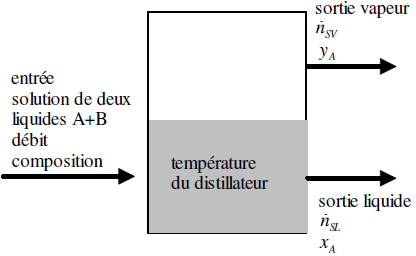
\includegraphics[scale=0.5]{images/distillation.png}\\
$EL$: entrée liquide\\
$SL$: sortie liquide\\
$SV$: sortie vapeur

\subsubsection{Débit molaire}
$$\dot{n}_{EL}= \dot{n}_{SL} + \dot{n}_{SV}$$
$$\underbrace{(x_{A,EL}\cdot \dot{n}_{EL})}_{EL} = \underbrace{(x_{A,SL} \cdot \dot{n}_{SL})}_{SL} + \underbrace{(y_{A,SV})\cdot \dot{n}_{SV}}_{SV}$$

\subsubsection{Fraction molaire dans la sortie vapeur}
En équilibre dans le distillateur
$$\underbrace{y_{A}}_{SV}=\frac{P_A}{P_A + P_B}=\underbrace{\frac{x_A \cdot \accentset{\circ}{P}_A}{x_A \cdot \accentset{\circ}{P}_A + x_B \cdot \accentset{\circ}{P}_B}}_{SL}$$

\subsubsection{Fraction massique dans la sortie (liquide ou vapeur)}
$$\% mas_{A} = \frac{y_{A} \times M_A}{y_{A} \times M_A + y_{B} \times M_B}$$

\subsubsection{Débit massique}
$$\dot{m}_{EL}= \dot{m}_{SL} + \dot{m}_{SV}$$
$$\underbrace{(\% mas_{A}\cdot \dot{m_{EL}})}_{EL} = \underbrace{(\% mas_{A} \cdot \dot{m}_{SL})}_{SL} + \underbrace{(\% mas_{A} \cdot \dot{m_{SV}})}_{SV}$$

%------------------------------------------
%------------------- Propriétés colligatives
%------------------------------------------
\section{Propriétés colligatives}
{\small *Pour les solutions formées de \textbf{solutés solides dans un solvant liquide}, les constantes sont dans le tableau 3.2}

\subsection{Diminution de la pression de vapeur}
$$P_{vapeur\ solution}=x_{solvant} \times \accentset{\circ}{P}_{solvant}$$

\subsection{Augmentation du point d'ébullition}
$$T_{b\ solution} = T_{b\ solvant} + k_b \times molalite$$

\subsection{Diminution du point de congélation}
$$T_{c\ solution} = T_{c\ solvant} - k_c \times molalite$$

\clearpage
%------------------------------------------
%------------------- Solutions liquides
%------------------------------------------
\section{Solutions liquides}
$$1ppm=\frac{1g\ constituant}{10^6g\ melange}$$
1g * 1000 = 1ppm\\
\textbf{Nombre de moles}
$$n=\frac{m}{M}$$
\textbf{Fraction massique}
$$\%mas = \frac{m_{compose}}{m_{total}}$$
\textbf{Fraction volumique}
$$\%vol = \frac{V_{compose}}{V_{total}}$$
\textbf{Fraction molaire}
$$x = \frac{n_{compose}}{n_{total}}$$
\textbf{Masse volumique}
$$\rho=\frac{m_{melange}}{V_{melange}}$$
\textbf{Concentration massique volumique}
$$cmasv=\frac{m_{compose}}{V_{solution}}\ g/L$$
\textbf{Concentration molaire volumique (molarité)}
$$[cmolv]=\frac{n_{compose}}{V_{solution}}\ mol/L$$
\textbf{Molarité en particules (molalité)}
$$m_p=\frac{n_{particules}}{m_{solvant}\ kg}\ mol/kg$$

%------------------------------------------
%------------------- Solubilité des gaz
%------------------------------------------
\section{Solubilité des gaz}
\textbf{Loi de Henry}
équilibre de solubilité d'un gaz dans l'eau:
$$[gaz]_{aq}=k_H \times P_{gaz}$$
$k_H$: tableau 3.3\\
$[gaz]_{aq}$: concentration molaire volumique du gaz dissous (mol/L)\\

$$n_{gaz}=\frac{p_{gaz} \cdot V_{gaz}}{R \cdot T}\ \textrm{, (V en $m^3$)}$$
$$n_{liquide}=p_{gaz}\cdot k_{H} \cdot V_{liquide}\ \textrm{, (V en litre)}$$
$$n_{tot}=n_{gaz} + n_{liquide}$$

%------------------------------------------
%------------------- DBO et traitement des eaux
%------------------------------------------
\section{DBO et traitement des eaux}

\subsection{Demande biochimique d'oxygène}
Masse d'oxygène (en mg) requise par les micro-organismes pour décomposer les matières biodégradables présentes dans un litre (1L) d'eau.

\subsection{Test normalisé}
On mesure la quatité d'oxygène au départ, puis après 5 jours

$$DBO = \frac{m_{O_2 debut} - m_{O_2 fin}}{V_{echantillon\ eau\ usee}}$$
{\footnotesize *$m$ en mg et $V$ en L}

\subsection{Traitement biologique des eaux usées}
$$\mathop{\dot{m}_{O_2}}_{\textrm{\scriptsize requis à l'entrée}} - \mathop{\dot{m}_{O_2}}_{\textrm{\scriptsize réellement fourni}} = \mathop{\dot{m}_{O_2}}_{\textrm{\scriptsize qui restera à fournir}}$$

\subsection{Bilan sur l'oxygène}
$$\mathop{\dot{m}_{O_2}}_{\textrm{\scriptsize requis à l'entrée}} = Q_{eau} \times DBO_{entree}$$
$$\mathop{\dot{m}_{O_2}}_{\textrm{\scriptsize qui restera à fournir}} = Q_{eau} \times DBO_{sortie}$$
$$\mathop{\dot{m}_{O_2}}_{\textrm{\scriptsize réellement fourni}} = \mathop{\dot{n}_{O_2}}_{\textrm{\scriptsize pompé par les surpresseurs}} \times \mathop{coefficient}_{\textrm{\scriptsize efficacité de la diffusion}} \times M_{O_2}$$

%------------------------------------------
%------------------- Exemples
%------------------------------------------
\clearpage
\section{Annexe: Exercices}

\subsection{Gaz et vapeurs}
\frame{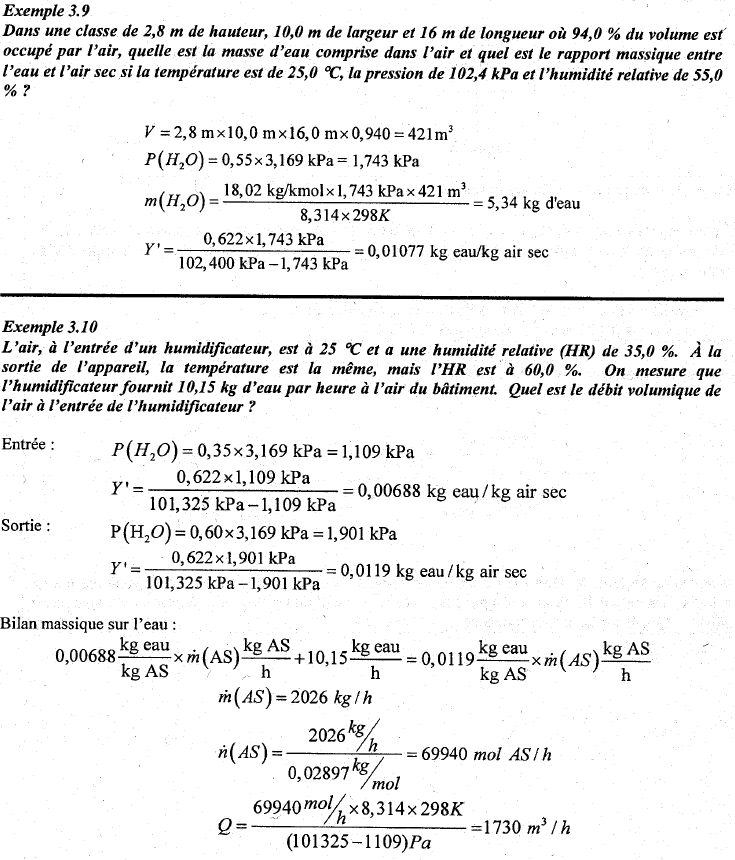
\includegraphics[width=0.5\textwidth]{images/01.png}}\\\\
\frame{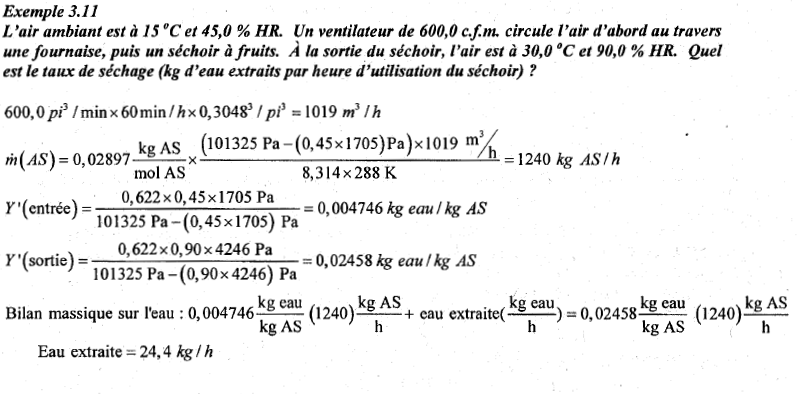
\includegraphics[width=0.5\textwidth]{images/02.png}}\\\\
\frame{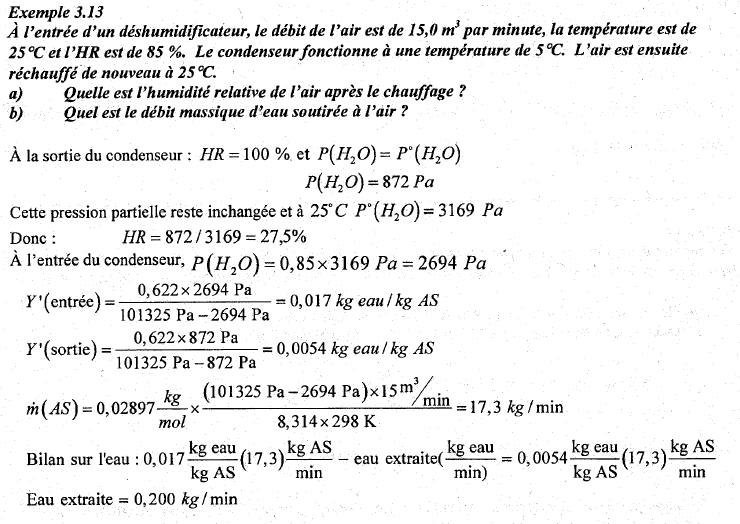
\includegraphics[width=0.5\textwidth]{images/04.png}}\newpage
\frame{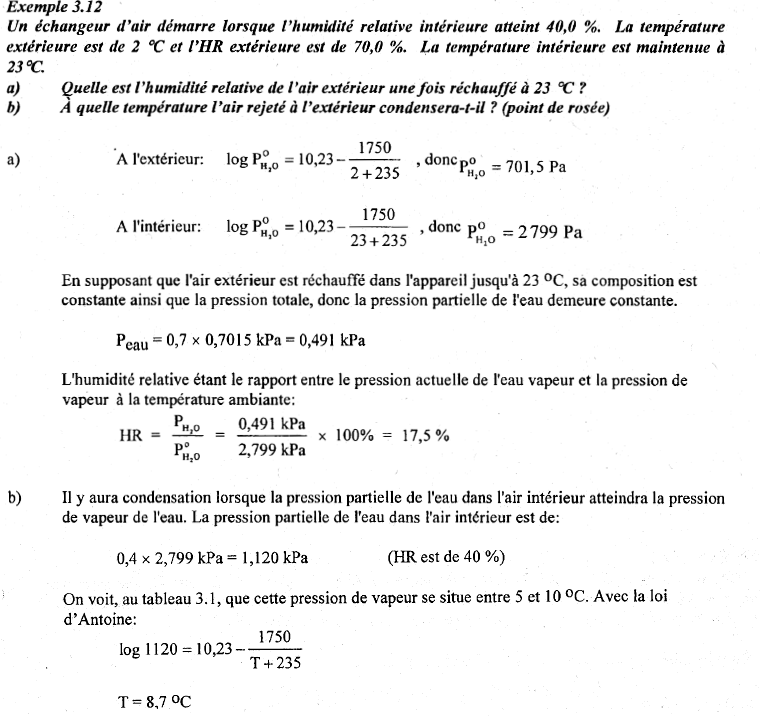
\includegraphics[width=0.5\textwidth]{images/03.png}}

\subsection{Réactions chimiques et stoechiométrie}
\frame{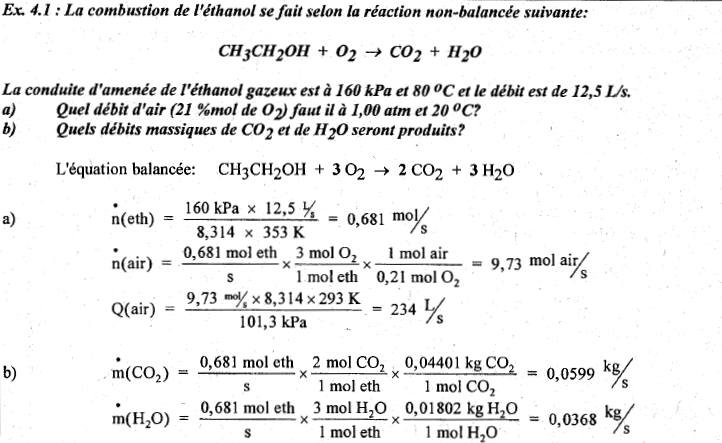
\includegraphics[width=0.5\textwidth]{images/05.png}}\\\\
\frame{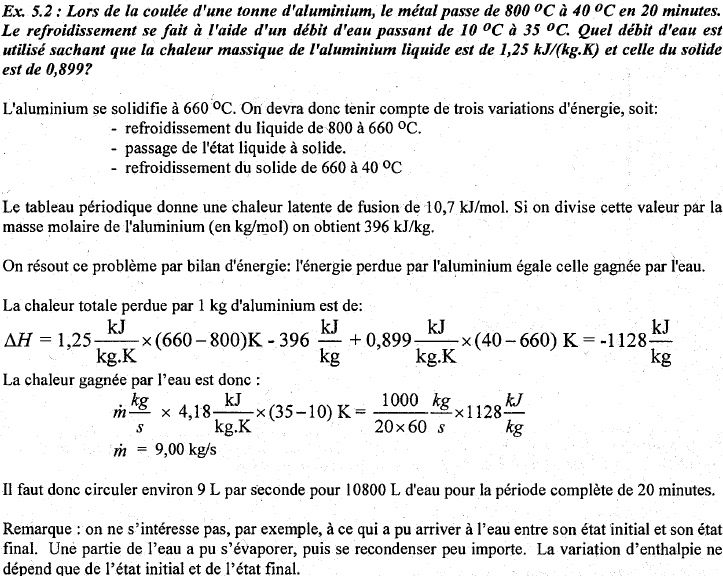
\includegraphics[width=0.5\textwidth]{images/06.png}}\\\\
\frame{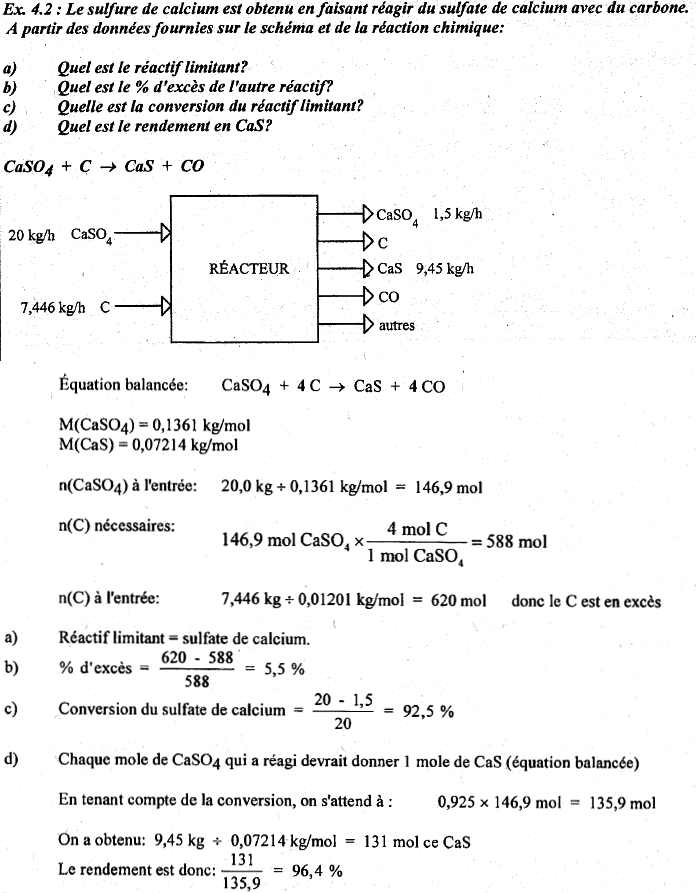
\includegraphics[width=0.5\textwidth]{images/ex_reaction_chimique.png}}

\subsection{Thermochimie}
\frame{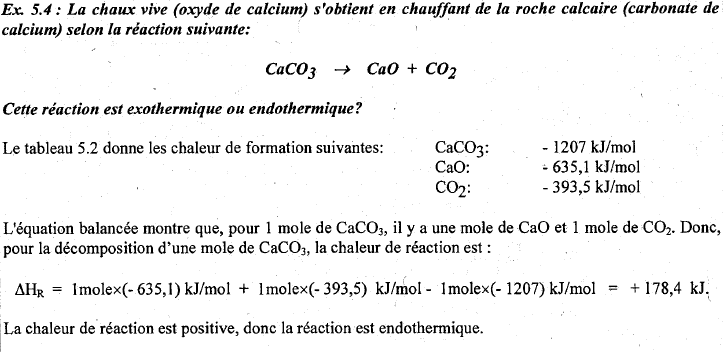
\includegraphics[width=0.5\textwidth]{images/07.png}}\newpage
\frame{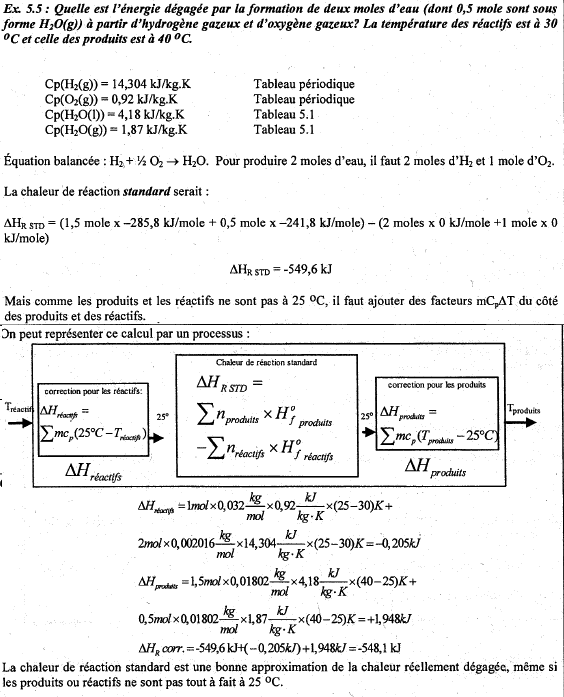
\includegraphics[width=0.5\textwidth]{images/08.png}}\\\\

\subsection{Combustion}
\frame{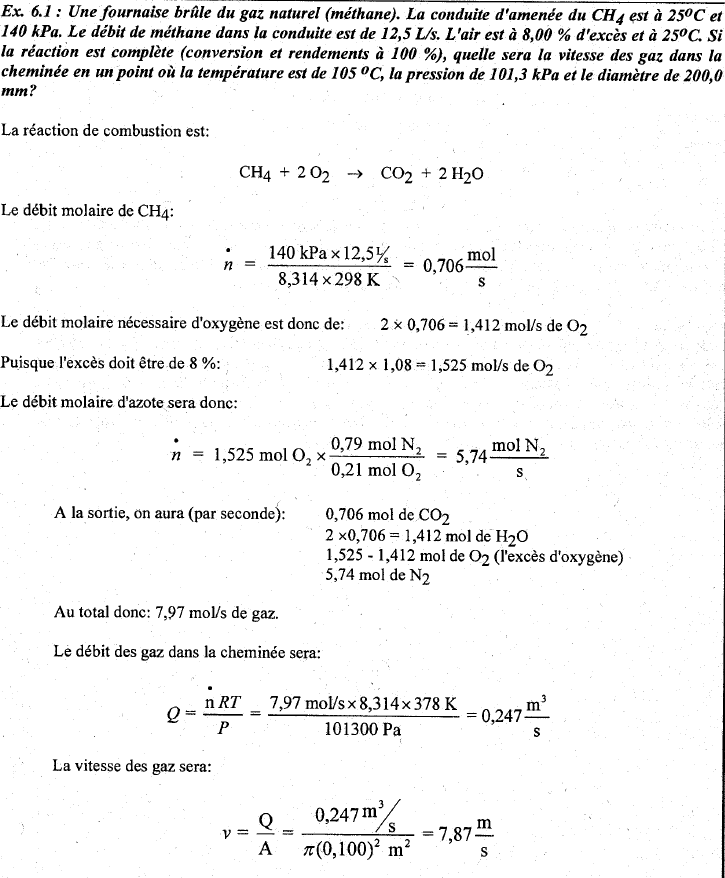
\includegraphics[width=0.5\textwidth]{images/09.png}}\\\\
\frame{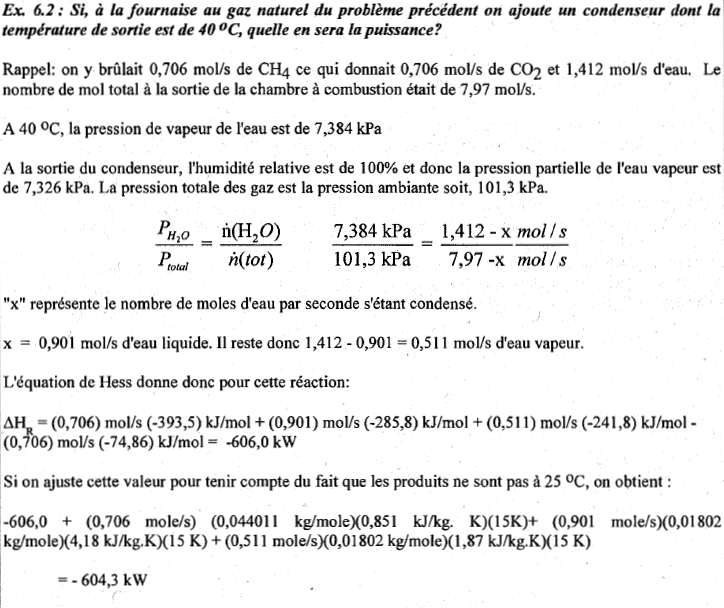
\includegraphics[width=0.5\textwidth]{images/10.png}}\newpage
\frame{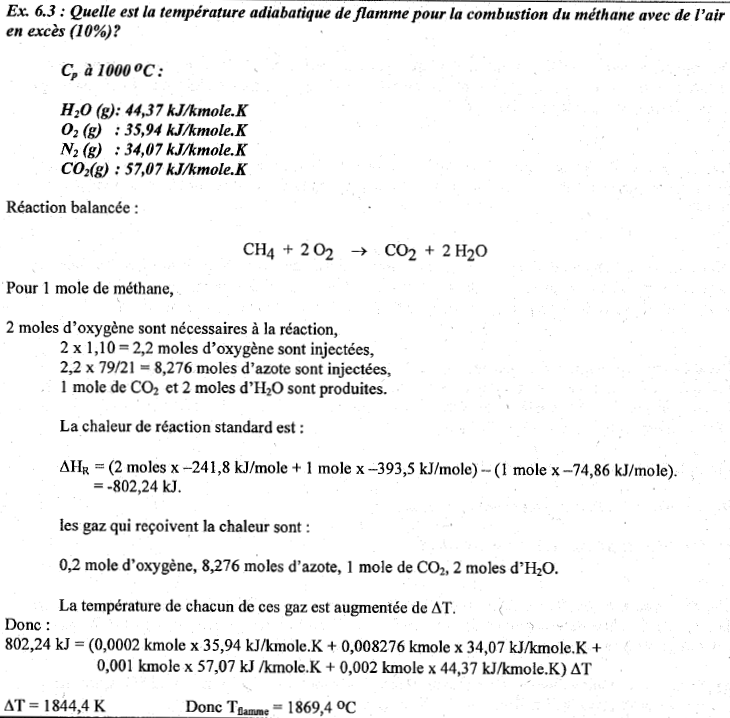
\includegraphics[width=0.5\textwidth]{images/11.png}}\\\\

\end{document}